\section{Methodology}

\section{Implementation}


\subsection{Code Schematic}

\begin{figure}[t]
\centering
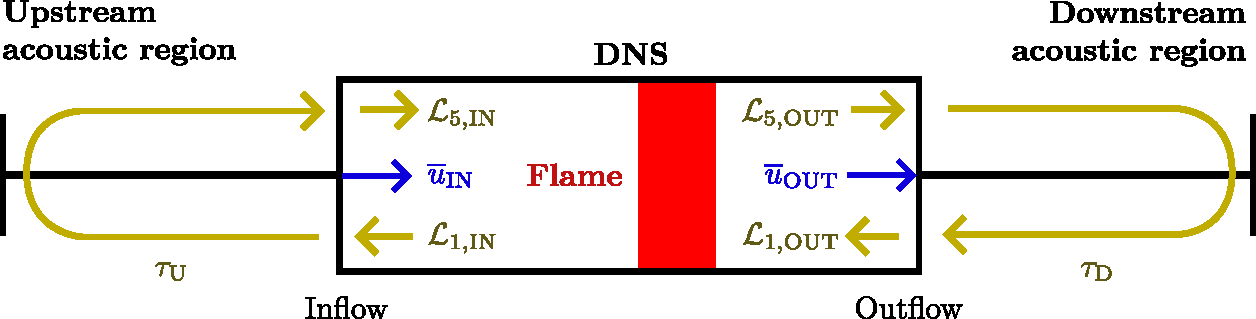
\includegraphics[scale=0.65]{assets/imgs/delay_bc_model.pdf}
\label{fig:delay-model}
\caption{MODEL OF DELAY BC. DELAY IS ONLY MODELLED VIA TIME SERIES OF L VALUES AS THEY LEAVE THE DNS DOMAIN.}
\end{figure}

\begin{figure}[t]
\centering
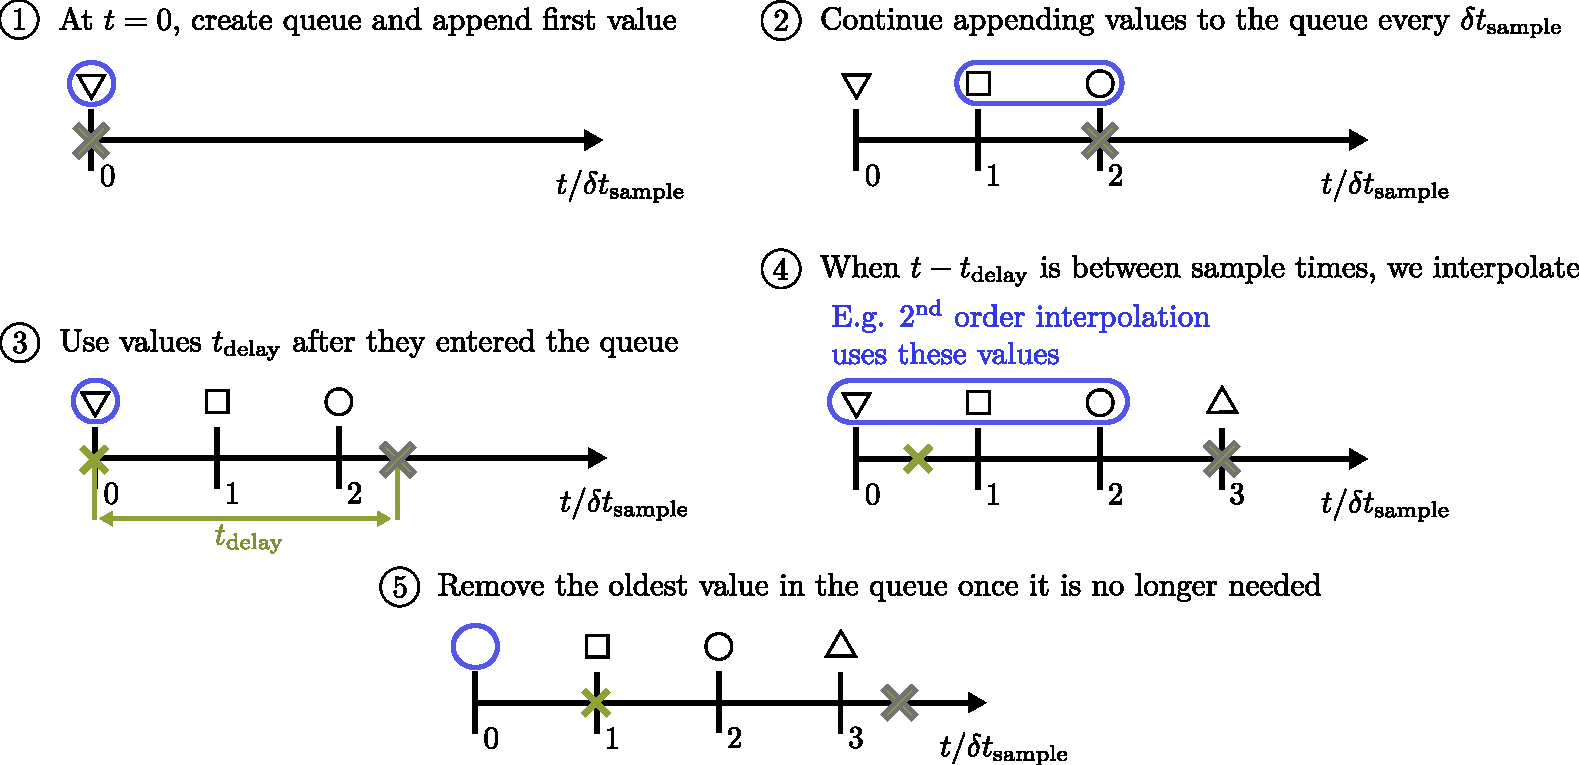
\includegraphics[scale=0.65]{assets/imgs/delay_bc_queue.pdf}
\label{fig:delay-queue}
\caption{HOW THE BOUNDARY SAMPLING AND DELAY WORK. WHAT DO SHAPES REPRESENT?? GREY CROSS IS CURRENT SIMULATION TIME, GOLD CROSS IS THAT TIME MINUS THE TIME DELAY. CHANGING TIME DELAY IS NOT SHOWN HERE.}
\end{figure}

\begin{figure}[t]
\centering
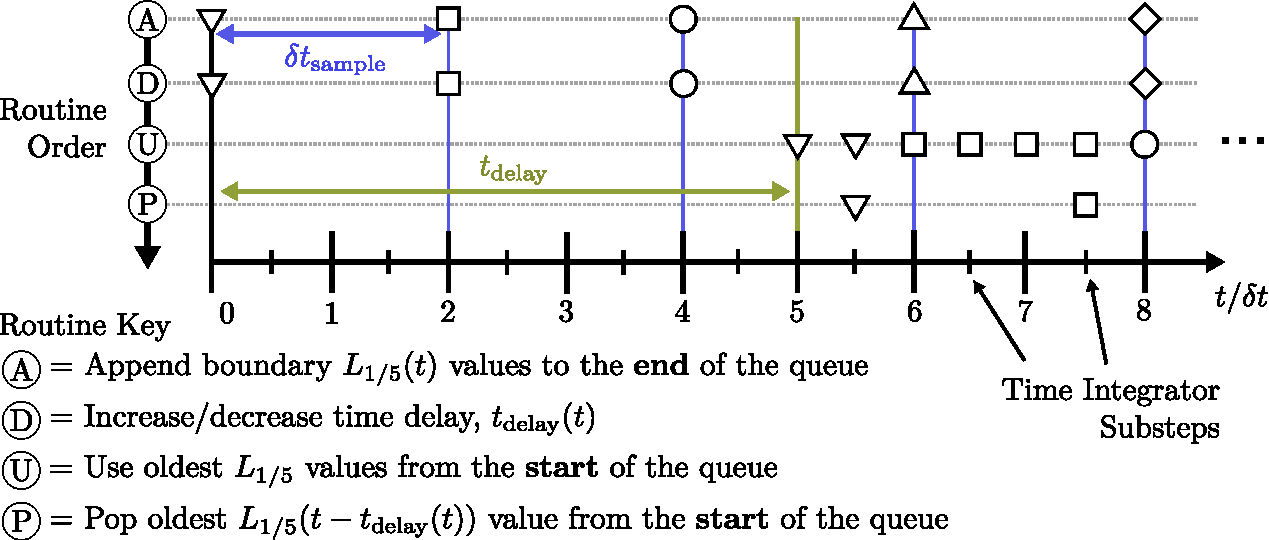
\includegraphics[scale=0.65]{assets/imgs/delay_bc_code_schematic.pdf}
\label{fig:schematic}
\caption{Schematic for delay BCs implemented into a multistage time integrator. ASSUMES CONSTANT TIME STEPS. TOP TO BOTTOM, LEFT TO RIGHT. BLUE SHOWS SAMPLE TIMES, GOLD SHOWS TIME DELAY}
\end{figure}


\begin{itemize}
\item Queues are filled with $L$ values as well as 
\end{itemize}



\subsection{Comparison with D-TDIBC}



\subsection{Overcoming Instabilities}



\subsection{Sampling Error}




